\begin{figure}[ht]
	\centering
	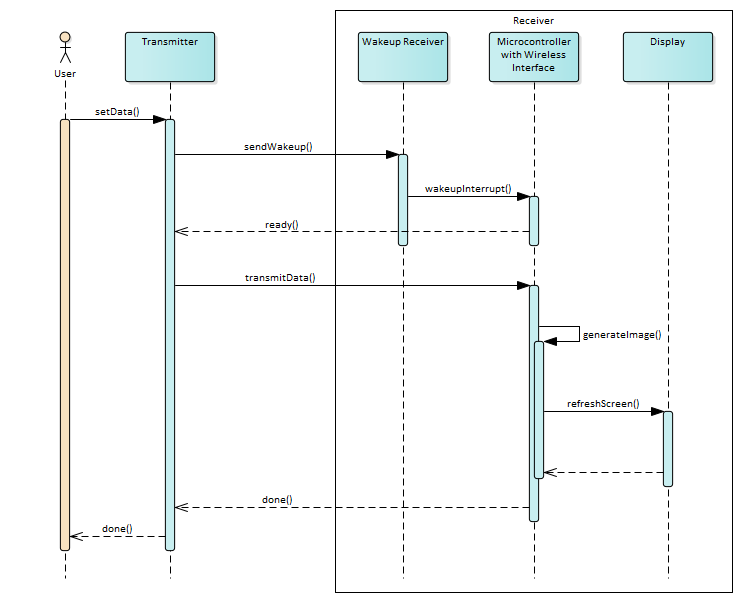
\includegraphics[width=0.9\textwidth]{4-development/software/graphics/1.png}
	\caption{not up to date sequence\label{software:sequence}}
\end{figure}

The software of the ULPWUR is separated in three different parts. 

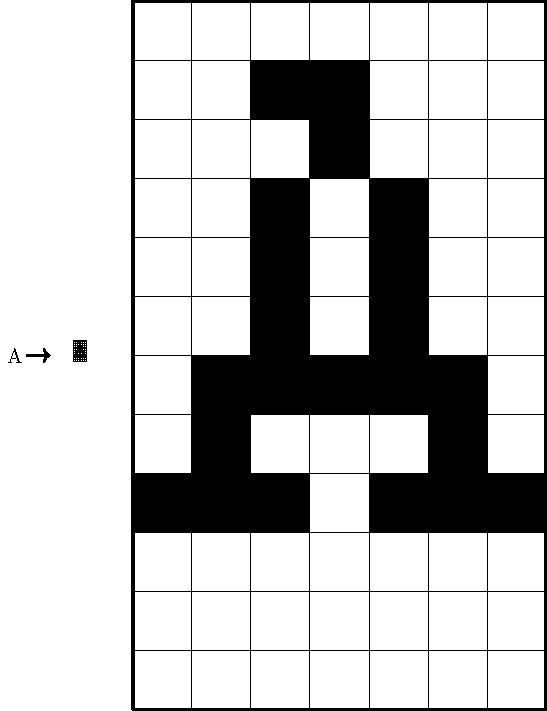
\includegraphics[scale=0.3]{4-development/software/graphics/font12.pdf}

\subsection{Receiver}

\subsubsection{Python-script}
\lstset{basicstyle=\footnotesize}
\lstdefinestyle{mystyle}{
	language=Python,
	basicstyle=\footnotesize\ttfamily,
	morekeywords={as},
	keywordstyle=\color{blue!50!black},
	stringstyle=\color{green!50!black},
	numberstyle=\color{red},
	emph={int,char,double,float,range, len},
	emphstyle=\color{violet}
}
\lstset{style=mystyle}

A short python script enables the user to send the data over an USB-port to the nRF52840.

%\lstinputlisting{4-development/software/code/WriteSection.py}

\subsubsection{nRF52840}


\subsection{Transceiver}